\section{Technology Assessment} % (fold)
\label{sec:technology_assessment}

According to the four types of prototypes in design science \cite{Johannesson:2014co}, our artifact was intended to be of the model type. A model can be used for supporting the construction of other prototypes, and hopefully our model can be reused by later projects. We wanted to come up with a design and then create a prototype that let us test different aspects of using low energy sensors for wireless ECG monitoring. Based on what we knew from previous literature we decided the following three aspects constituted the baseline functional tests that would answer our research questions:
\begin{itemize}
	
	\item End to end latency
	\item Battery life
	\item Maximum throughput
  
\end{itemize}
\noindent
We validate our proposed design through a working prototype. Our prototype takes the form of a test bed that can be used to address the items listed above experimentally. This section starts with a discussion on different technical and architectural alternatives, and the decisions that went into it. Later we describe how the base of the testbed was implemented, before we customized it in order to evaluate the baseline functional tests.

\subsection{System architecture} % (fold)
\label{sub:system_architecture}

As mentioned in Section~\ref{sec:literature_review}, different architectures has been proposed and discussed in large by previous research. A general solution to how WBANs should be organized in relation to existing infrastructure do not exist, and is an important research topic. Mainly two different architectures have been discussed earlier: One where the WBAN routes all traffic through a personal gateway, and another one where it directs the traffic directly to an access point. See Figure~\ref{fig:architecture}. In \cite{Shahamabadi:2013df} a third approach is proposed. This merges the two former ones, where WBAN data is sent directly to the access point, while the personal gateway is given the responsibility of coordinating mobility issues like exchanging handover messages on behalf of the WBAN. In the following section, we will compare the first two approaches as seen in Figure~\ref{fig:architecture}.

\begin{figure}[H]
\centering
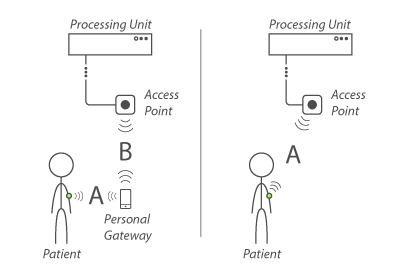
\includegraphics[scale=0.75]{img/figures/architecture.png}
\caption{Here A represents Bluetooth Smart while B is 802.11}
\label{fig:architecture}
\end{figure}

\noindent
Based on what we know about the existing telemetry systems deployed today and the research on WBAN sensor devices, it is improbable that all sensory devices will be (A) developed by the same manufacturer, and (B) that they all communicate over the same physical medium. The question of data interoperability is an interesting topic, because of the technical constraints imposed by the small sensors. At what point in the pipeline do we enforce the standardized data formats for exchanging medical information? In general, we believe this should be done as early as possible in the process, preferably at the node level. However, we want to highlight two arguments to why this might not be optimal: Although there has been invested a lot of effort by standardization organizations like HL7 and OpenEHR the last 30 years, data standardization in health care remains a challenge - not only across institutions, but also between information systems located at the same hospital. Based on this, requiring standardized formats with reduced footprint, optimized for constrained sensory devices, might not be realistic. As mentioned in Sect. 3, organizations like Continua are currently trying to bridge this gap, but with a primary focus on personal health technology, not clinical. This is a topic that need more research.

Another argument to why it might not be feasible to enforce todays standardized data formats for physiological measurements at node level, is related to the technical constraints of these devices. In order to keep the energy consumption down, overhead is reduced and as little data as possible is sent. This is especially true for continuous, streaming data sources like ECG. The approach Continua and ISO/IEEE has to this problem is to make smaller standardized measurement data formats tailored for constrained devices. Then they specify how these data formats should be transformed or mapped onto richer, data formats with a larger space footprint at a gateway level.

Relating this to the architectures discussed in previous research, we identify certain practical advantages of routing all traffic trough the personal gateway: Making a personal gateway compatible with a given sensor and its manufacturer specific or protocol specific\footnote{ If standardized data formats are used} data format is a trivial task through software applications installed on the personal gateway device. The same triviality does not hold for a smart access point/boarder router wanting to transform the data into a richer, standardized data format. In a reality where a standardized data format is not implemented by every sensor node, giving an access point the role as a WBAN sink, as suggested by \cite{DrAmirMohammadRahmani:2014vx} seems highly impractical: All access points in a roaming environment would have to be compatible with custom data formats from several WBAN sensors carried by a multitude of patients. In this scenario, we only see smart gateways/access points being able to fulfill this data processing and transformation responsibility if standardized data formats for every physiological measurement is implemented at WBAN node level.

Based on these considerations, our proposed architecture consist of the following parts: a single sensor node simulating a patient ECG device, a personal mobile gateway acting as a WBAN sink to be carried by the patient, a monitoring server available on a local or remote network together with a client interface for remote monitoring. In order to reduce the scope and complexity we have decided to only include one node in our prototype. This is a clear limitation with our prototype and study, as we only consider a single-hop star network topology in instead of a mesh topology, which is proven to be the most effective topology for WBANs. One concern here might be that Bluetooth does not currently support mesh networks, but as as Feb. 24 2015 the Bluetooth SIG formally announced formation of the Bluetooth Smart Mesh Working Group \cite{bt:sig:mesh}, and we operate under the assumption that this will be supported in future versions. The gateway should have the responsibility of routing the sampled data from the WBAN to an external endpoint. In accordance with Continua's guidelines, we also propose that the gateway enforce interoperability by transforming the data into a standardized medical format. But how can this be accomplished in a multi sensor, multi manufacturer environment? 

We believe this can be solved by using the repository architectural pattern. The gateway application could be extendable with different ``profiles'' to accommodate for both different manufacturers,  different communication protocols, and different data formats. These profiles would be installed from a repository, central to a hostpial, region or country depending on the supported data formats. The profiles would contain a mapping between a given sensor peripheral and the preferred output data format compliant with the monitoring system a given hostpial was using. This way, the hospital could support a growing amount of sensor peripherals, independent of sensor manufacturer.

See Table~\ref{tab:system_components} for a formal description of each component of our prototype.

% TODO create table system_components

An overview of the different prototype components:
\begin{itemize}

  \item[\textbf{Node:}] A node is the sensory device that does one or more physiological measurements and communicates it wirelessly to either another node or to a sink in the WBAN. In order to achieve wearability the nodes has to be as small as possible. Batteries are often the largest part of today’s sensory nodes and the biggest energy consumer is typically the antenna \cite{Ullah:2010ci}.

  % \item[\textbf{WBAN:}] Multiple nodes connected together constitute the wireless body area network (WBAN). The network topology of these vary depending on the communication protocol between the nodes, but they are typically organized as single hop stars, or multi-hop mesh networks \cite{Anonymous:6F6UBBK9}. Desirable qualities in a WBAN is a low energy PHY layer, and a flexible MAC protocol capable of doing smart routing and the ability to be self organizing \cite{Anonymous:XKViPHhV} \cite{Anonymous:OEjzuKTe}.

  \item[\textbf{Personal gateway:}] In previous literature this tier in the patient monitoring stack is also called a Personal Server (PS) or a WBAN sink. This can be a touch device with a graphical user interface, a tele health station, or just a dedicated sink in the WBAN with a larger battery. Because of the low energy consumption of the nodes, you typically need to facilitate communication between the WBAN and a boarder router with some device that has more battery capacity, a stronger antenna and that is easier to replace on a frequent basis. For the remainder of this thesis we will assume the personal gateway is a feature rich touch device, with a graphical user interface like the Samsung Galaxy S6.

  % \item[\textbf{Boarder router:}] The border router can be categorized as a end node in a local area network providing access network access for proprietary devices through one or more wireless networking interfaces. Based on the network configuration and overall architecture of the monitoring system this router may have different responsibilities. A smart-gateway can for example provide additional services specialized for sensory data. These services can include but are not limited to local caching, pre-processing and on-demand-processing, WBAN discovery, localization and more \cite{DrAmirMohammadRahmani:2014vx}.

  \item[\textbf{HIS:}] Hospital information system. This is a common term for the various types of information systems at hospitals. The way these are implemented and used varies from across borders, regions, and even between different departments within the same hospital. Because of this invariance in systems and practice, interoperability across communication protocols and data formats is of outmost importance. For the remainder of this thesis we will discuss only one HIS, namely the monitoring central. This is responsible for collecting, processing and storing and serving sensor data to clients.

\end{itemize}

% TODO Ha med et diagram over arkitekturen slik vi foreslår den

% subsection system_architecture (end)

\subsection{Sensor Node} % (fold)
\label{sub:node}

While deciding on what platform to use for the prototype of our proposed design, we looked through a wide array of different System on a Chip (SoC) solutions and boards enabling rapid prototyping and testing with Bluetooth Low Energy. In order to increase reproducibility and ease later projects, an overview of the different development kits we evaluated has been included in Appendix~\ref{sec:soc_considerations}.

Most of the relevant development kits we evaluated were based on one of the Nordic nRF51-series chips \cite{newRef:36, newRef:36:2}. Because hardware design and development was uncharted territory for the researchers, the availability of online communities and documentation was a critical factor when assessing/deciding on what development kit to base our prototype on. Nordic themselves has a thriving community on their Stack Overflow inspired developer zone \cite{newRef:50}, which has at the time of writing has over 13,800 questions asked. Because of this we decided a development kit based on the  nRF51822 chip was our best alternative. Because Nordic Semiconductor also offer their own development kits, we decided to use their boards as the basis of our prototype, reducing the number of external dependencies.

In terms of software development on these different boards, we investigated the different IoT operating systems and assessed the feasibility of using these for our purpose. After a quick survey, the small RiotOS \cite{Anonymous:a1din1ZK}, running on only 1.5kB RAM and 5kB of ROM, looked like the most promising alternative. A comparison of the major operating systems for IoT-applications can be found at \cite{Anonymous:a1din1ZK}. For our project however, it was concluded that the node functionality would be limited and specialized rather than general. Hence, adding a dedicated operating system to our already growing technology stack would impose more risk to our project. It should also be mentioned that this technology and the platforms that are being built around them are not very mature: The seeds for RiotOS were planted less than 10 years ago as it started out as an operating system for wireless sensor networks in Germany in 2008 \cite{newRef:52}. An example of this lack of maturity, is that we have yet to find a RiotOS library for accessing the Bluetooth stack on nRF51822 trough SoftDevices.

Due to the increasing risk and complexity more dependencies add to the development, we dropped support for 6LoWPAN, although this is an important advance for network interoperability in low energy devices. There was an interest for this when we started the project, but a concurrent research project investigating the practical limitations of using IPv6 enabled Bluetooth Smart (6LoWPAN) technology, was already in progress at the Department of Telematics.


\subsubsection{Implementation} % (fold)
\label{ssub:implementation}

The first prototype iteration used a Nordic nRF51 evaluation kit from 2013, which supported Bluetooth Smart version 4.0 trough a software stack Nordic calls SoftDevices. A SoftDevice is a precompiled and linked binary that implements the Bluetooth protocol stack for NRF51 boards. Because of the board's relative old age (development in this area happens at a rapid pace) the latest Nordic SDK\footnote{ The Nordic nRF5 SDK forms the foundation of what you need of drivers, libraries SoftDevices and code examples to develop your own low-energy Bluetooth, ANT product} support for this board was version 6, while the most recent SDK is at version 10. This turned out to cause a lot of compatibility problems, and the development process was tedious: We had to flash both SoftDevice and our own compiled software onto the board manually using Segger's J-Link software. In addition to this, the J-Link debugging options were not supported on our development system.

Because of the compatibility/legacy issues we had with the node in our initial prototype, we decided to replace the 2013 evaluation kit for a nRF51 Development Kit originally released late 2014 \cite{newRef:53}. This board supports a newer SDK (version 8), two new SoftDevices and ARM's mBED development platform \cite{newRef:54} The latter was crucial as it drastically eased the process of compiling and installing software on the development board. mBED is a online development platform for embedded devices developed and maintained by Arm \cite{newRef:55} along with partners and contributors. It solves the problem of setting up an correct environment for compiling C++ code specific to a given development board, by building and compiling programs in the cloud. This means they maintain and keep track of all dependencies and environment configurations needed for correctly building and compiling code specific to a given board before making a binary file available for download. An mBED enabled board connected to your computer via USB will be available as a mass storage device. In order to install the software, you simply drag the bundled binaries over to the mass storage device, and the compiled software will auto-install. 

While the development process was eased, programming ARM Cortex M is still complicated, and so is Bluetooth Low Energy. Simulating ECG data is also a non-trivial task, and based on these three factors we decided to use as much available code for the board programming as possible.

In order to simulate the ECG data stream on the board, different existing ECG simulators written in C++ were considered \cite{newRef:56, newRef:56:1, newRef:56:2}. We decided to go for ECGSYN, a realistic ECG waveform generator created at Oxford and MIT \cite{newRef:56:2}. This is a flexible program that let us customize sampling frequency and mean heart rate among other things. ECGSYN generates a synthesized ECG signal based on algorithms described in \cite{newRef:58}. Se figure Listing~\ref{lst:ecgsyn:terminal} for an overview of the different adjustable parameters.

\begin{lstlisting}[caption={ECGSYN Commando Line Interface (CLI)}, label={lst:ecgsyn:terminal}, basicstyle=\small]

    >> ecgsyn $
    ECGSYN: A program for generating a realistic synthetic ECG
    Copyright (c) 2003 by Patrick McSharry & Gari Clifford. All rights reserved.
     
    O Name of output data file                 "ecgsyn.dat"
    n Approximate number of heart beats        256
    s ECG sampling frequency [Hz]              256
    S Internal Sampling frequency [Hz]         256
    a Amplitude of additive uniform noise [mV] 0
    h Heart rate mean [bpm]                    60
    H Heart rate standard deviation [bpm]      1
    f Low frequency [Hz]                       0.1
    F High frequency [Hz]                      0.25
    v Low frequency standard deviation [Hz]    0.01
    V High frequency standard deviation [Hz]   0.01
    q LF/HF ratio                              0.5
    R Seed                                     1
    (Type ? for Help)
    ->

\end{lstlisting}

\subsubsection{Maximum Throughput} % (fold)
\label{ssub:maximum_throughput}

Because experience with embedded software development was limited, we did some preliminary research on max throughput on Bluetooth Smart, before starting the customization and implementation of the ECGYN software on the development board. As mentioned in Section~\ref{sec:literature_review}, Bluetooth Smart specifies the theoretical max throughput to be 1 Mbit/s. However there are always factors limiting this theoretical capacity. In the following section will elaborate on these limiting factors, and comparing our findings with the minimum requirements of clinical ECG.

Once a Bluetooth Smart connection is established between two devices, the connection parameters \cite{newRef:59} control the frequency at which data can be sent between the two devices\footnote{ In this example the mobile gateway acts the role of the client, and the wireless sensor acts the role of the server - the one with data.}. The two connection parameters of interest to us are, minimum and maximum connection interval, which specify the minimum and maximum rate at which the client will ask for data from the server. By the Bluetooth SIG specification, both fields have an allowed minimum and maximum value of 6 and 3200. By multiplying these values by 1.25ms we get the highest and the lowest frequency at which a central may ask for data: 7,5ms and 4s (4000ms).

The GATT protocol specifies different commands for the client to get information about the server. Among these, GATT offers notifications and indications. In high-throughput applications a client can request/register a notification on a given characteristic. This means that the server will send a notification containing maximum 20 Byte of user data to the client whenever data becomes available. These notifications are buffered by the SoftDevice and ACK-ed in the link layer. The Bluetooth specification allows for up to 6 packets to be sent per connection interval, but this number may vary between different implementations. This gives the following formula for calculating max throughput:

\[
\frac{1000\: ms/s}{CI}\: \times\: PPI\: \times\: BPP\: \times\: 8\: bits/byte = Throughput
\]

\newline
\noindent
Here, \texttt{CI} is connection interval, \texttt{PPI} is packets per interval, and \texttt{BPP} represents the number of bytes sent per packet. Because packets per interval and the bytes per packet may vary between devices and operating systems, the maximum throughput over a Bluetooth Low Energy link is relative. However, maximizing the allowed values above, we get the following result: 
\[
\frac{1000\: ms/s}{7,5ms}\: \times\: 6\: packets\: \times\: 20\:bytes/packet\: \times\: 8\: bits/byte = 128\:Kbit/s
\]
\newline
\noindent
This is substantially lower than the advertised 1Mbit/s. In Table~\ref{tab:ble_device_throughput} we present calculated throughputs for different devices based on their implementation of the Bluetooth specification.

% Please add the following required packages to your document preamble:
% \usepackage{booktabs}
\begin{table}[]
\centering
\caption{Throughput on different devices.}
\label{tab:ble_device_throughput}
\begin{tabular}{@{}lrccr@{}}
\toprule
\textbf{Device}   & \textbf{Interval (i)} & \textbf{Packets/i} & \textbf{Bytes in packet} & \textbf{Throughput} \\ \midrule
Optimal	          & 7,5 ms	  & 6	  & 20 Byte	  & 125 kbit/s \\
iPhone	          & 30,0 ms	  & 4	  & 20 Byte	  & 21 kbit/s   \\
iPhone HID	      & 11,25 ms	& 4	  & 20 Byte	  & 56 kbit/s \\
Macbook pro	      & 11,25 ms	& 4	  & 20 Byte	  & 56 kbit/s \\
Android (Nexus 4)	& 7,5 ms	  & 6	  & 20 Byte	  & 125 kbit/s  \\ \bottomrule
\end{tabular}
\end{table}


To confirm this discovery we installed some firmware \cite{nordic:throughputtest} to see if we indeed could achieve the 128 Kbit/s throughput. However, our LG G4 test device did not support this optimized Bluetooth configuration, and dropped the connection as soon as the throughput test started. This proves that there are even differences between Android devices, as the operating system \emph{should} support the optimal configuration. Based on the discoveries made above we decided not to implement ECGSYN for simulating streaming ECG from the node. The reason for this is addressed in Section~\ref{ssub:throughput}. For the end-to-end latency experiment, we based our code on the BLE\_HeartRate repository \cite{mbed:bleheartrate} published by the Bluetooth Low Energy team at the mBed platform. The details of this implementation will be addressed in Section~\ref{ssub:end_to_end_latency}.

% subsection node (end)

\subsection{Gateway} % (fold)
\label{sub:gateway}

% TODO Create figure: tab:ble_device_throughput from excel sheet

Although creating a user friendly application was not part of the scope of this project, we believe some thoughts on usability and context should be put into the creation of any artifact. We did not want to hard code the UUID address of Nordic chip into the gateway and connecting the data stream with a static endpoint address. Therefore we have created what we consider to be the bare minimum of a personal WBAN gateway user interface. The functional requirements of this user interface can be found in Table~\ref{tab:gatewayRequirements}.

\begin{table}[]
\centering
\caption{Personal Gateway Functional Requirements}
\label{tab:gatewayRequirements}
\begin{tabular}{|l|l|l|}
\hline
\textbf{FR\#} & \multicolumn{1}{c|}{\textbf{Description}} & \multicolumn{1}{c|}{\textbf{Priority}} \\ \hline
1             & Add new sensor                            & High                                   \\ \hline
1.1           & \ \ \ \ Scan for nearby BLE devices               & High                                   \\ \hline
1.2           & \ \ \ \ Select endpoint                           & High                                   \\ \hline
1.3           & \ \ \ \ Select BLE Characteristic                 & Medium                                 \\ \hline
1.4           & \ \ \ \ Add new endpoints                         & Low                                 \\ \hline
1.5           & \ \ \ \ Give each sensor a name                   & Low                                    \\ \hline
2             & Ability to test sensor connection         & Medium                                 \\ \hline
3             & Ability  to test endpoint connection      & Medium                                 \\ \hline
4             & List all sensor nodes                     & Low                                    \\ \hline
\end{tabular}
\end{table}

With an architecture dependent on a personal mobile gateway we chose a technology that was in accordance with our mission statement: available and open. The Android platform is not only more open than it's counterparts, but also supports higher throughput as seen in Table~\ref{tab:ble_device_throughput}.
The gateway would ideally be a multi-purpose touch device with a rich user interface, enabling an easy and practical way of setting up and configuring the wireless sensors a patient would be equipped with. Although outside the scope of this project, some thought have gone into the practicalities of setting up and managing a network of wireless sensor nodes. For further research we recommend looking into using Near Field Communication (NFC) technology for physically conducting events such as \emph{(A)} pairing sensors, \emph{(B)} connecting the gateway to the WBAN and \emph{(C)} authenticating medical professionals and patients on the personal gateway. We believe these are all use cases where an active NFC chip could drastically improve the user experience, but the subject need more research.

In the following section we will describe how we approached the implementation of the gateway application. Because we only intended to make a prototype, some details will be kept out for brevity. 

\subsubsection{User interface} % (fold)
\label{ssub:the_user_interface}

The functional requirements were prioritized and we developed the user interface in a iterative fashion as more functionality gradually were added. The resulting user interface is not user tested as this was outside the scope of this project. The ``front-end'' of the application consist of two simple views, as seen in Figure~\ref{fig:android_frontend}. In Android, a ``view'' is called an Activity. As the application is opened the user is presented with a list of sensors connected to the gateway. Clicking either a sensor or the plus sign in the downright corner brings the user to the next screen, where you can either modify the existing device or add a new one. 

The application has prioritized functionality over reliability, but still some basic error handling and connection tests are implemented. When connecting to both a Bluetooth Smart sensor and endpoint, the application tests the connection. How this is implemented is described in Section~\ref{ssub:bluetooth_module} and \ref{ssub:endpoint_module}. When both sensor and endpoint is selected, the user is able to activate the routing of the data by clicking on activate. The user should then be navigated back to the overview of previously added devices.

% subsubsection the_user_interface (end)

\subsubsection{Bluetooth Module} % (fold)
\label{ssub:bluetooth_module}

% TODO mention test

We have split the Bluetooth functionality out in a separate Android service. Having a loosely coupled application makes it easier to extend. Android services run in a separate background thread, which is important as makes the gateway continue to receive data after the application is minimized.

Having structured the code this way, a future version of the application could replace the Bluetooth service with, say a Zigbee service, if the device supported that interface.

We set up the scanning code to only look for low energy devices, and (as of now) the gateway application will only subscribe to the Heart-Rate characteristic. A previous version of the application made it possible to select what Bluetooth characteristic you wanted to receive notifications on\footnote{ This is Bluetooth jargon for subscribing to a certain data value} when adding the device. We removed this for the benefit of automatically selecting the heart rate characteristic. This was done both for usability\footnote{ As we had already set up the sensor node code to only write data to the heart rate characteristic, it was unnecessary to select the characteristic whenever we connected to it.} and because we believe that in a multi-vendor environment, sensor specific details\footnote{ as what characteristics to subscribe to are and other metadata} should be available in a remote repository, as mentioned in \ref{sub:system_architecture}. This will be further discussed in Chapter \ref{sec:discussion}.

The Android SDK supplies interfaces and example code for creating a BLE applications. In our case, the \code{BluetoothLeService} class sets up the necessary methods to initialize, connect and disconnect to a BLE device. The class can list supported characteristics and read a given characteristic as well as handling the service specific functionality, such as broadcasting data from Bluetooth notifications to other services/activities. Because our use cases only involved a one way data flow between the sensor node and gateway, we did not implement functionality such as writing data back to a given characteristic. In addition to this, the class also handles callbacks that Android's Bluetooth library execute when it is finished with a given action, such as scanning for devices, or on connection changes. The latter is how we test the connection in the \code{NewDevice} class. When the callback for \code{onConnectionStateChange} is executed, the Bluetooth service will broadcast an update, which the \code{NewDevice} activity listens for. These updates will contain one of the following identifying strings:\\
\newline
\noindent\code{
  ``iot\_gateway.ACTION\_GATT\_CONNECTED'';\\
  ``iot\_gateway.ACTION\_GATT\_DISCONNECTED'';\\
  ``iot\_gateway.ACTION\_GATT\_SERVICES\_DISCOVERED'';\\
  ``iot\_gateway.ACTION\_DATA\_AVAILABLE'';\\
  ``iot\_gateway.EXTRA\_DATA'';\\}
\\
\noindent
Based on these messages the \code{NewDevice} activity handles the event. Every callback we have implemented broadcasts an update, and the \code{EXTRA\_DATA} identification is used when the callback \code{onCharacteristicChanged} is executed. In our case this means that the \code{HEART\_RATE\_MEASUREMENT} characteristic is changed, since we set up the sensor node to change data on that characteristic in a given interval.

% subsubsection bluetooth_module (end)

\subsubsection{Endpoint module} % (fold)
\label{ssub:endpoint_module}

The endpoint module extends the Android-DDP\cite{android:ddp} library released under Apache License, Version 2.0. This library makes it easy to interact with a Meteor server, which is described further in~\ref{sub:server}. Because of how we did the server implementation, we used the library to connect to a WebSocket endpoint created by the Meteor server.
Although the endpoint module also was planned as an individual module, we never finished refactoring all endpoint functionality out to the \code{MeteorHandler} class which ideally would extend as an Android Service. This had some implications our experiments, which is addressed in Section~\ref{ssub:end_to_end_latency}.
As an intermediate step, we first implemented the DDP-library directly in the \cite{NewDevice} activity. We set it up as a instance-wide private object, that after first being set up, is available in every method. This was done in order to speed up development, and intended this to be refactored out of the Activity at a later stage. When initializing connection with \code{mMeteor.connect()} one of two callbacks defined in the MeteorCallback interface are executed, \code{onConnect()} or  \code{onDisconnect()}. When the connection is tested and active we pass data directly to the Meteor endpoint by calling \code{mMeteor.call("addData")} in the \code{BroadcastReceiver} method. As mentioned, the \code{BroadcastReceiver} listens for data from the Bluetooth service.

% subsubsection endpoint_module (end)

% subsection gateway (end)

\subsection{Server} % (fold)
\label{sub:server}

Inspired by \cite{Thelen:2014ew} and informed of the development within the standardization communities like (HL7 FHIR), we decided to mock up a monitoring central using web technologies. In addition to vastly simplify product development for a manufacturer, using web technologies also enables rapid prototyping for small research teams with little resources. As seen in Table~\ref{fig:serverRequirements}, functional requirements of the server prototype was limited. Based on experience with similar technology we decided to write the server software in Javascript. Contrary to it's young age, this is a programming language that has matured a lot over the last couple of years, and is today the most popular technology for full-stack developers \cite{so:survey:results}.

% TODO create table tab:serverRequirements

Because of the simple requirements and limited timespan available building the monitoring server, it was decided to utilize a development platform called Meteor. Meteor \cite{meteor} is an open source platform for developing web and mobile applications based on NodeJS. It comes with MongoDB database support out of the box, and its own data managing layer. This layer is based on a protocol they call Distributed Data Protocol (DDP), which uses WebSockets as a lower layer message transport. DDP implements the publish-subscribe messaging pattern, which lets clients publish and subscribe to data collections over WebSockets \cite{ddp:github}. This functionality was ideal for this project as it made us set up an endpoint where the gateway could route data from the sensor to the server in short time. When this data arrives at the server and is inserted in the database, Meteor will automatically synchronize the updates with all of it's clients that are subscribing to that data source. This new way of structuring web applications, is often called \textit{connected-client} or \textit{cloud client}, and it differs from the classic stateless request-response client-server architecture by synchronizing all clients immediately without the need for refreshing\footnote{ This is all part of a larger paradigm shift, where \textit{data} is sent the wire instead of documents (such as files).}.

It should be noted that WebSockets make use of TCP at the transport layer. Alensanco and Garcia concluded TCP was not suitable for real-time ECG transmission in a wide area network \cite{Alesanco:2010kc}. They suggested UDP as a more suitable transport layer protocol, but they were transmitting data over a 3G network. Out prototype is connected to local area network over a WiFi link, offering substantial network speeds and reliability over telecommunication networks.

In accordance with use case \textsc{UC2.2}, we designed and implemented a client interface for medical professionals to access the ECG data streams. Technically speaking, we wrote the client view using Blaze, Meteor's frontend rendering system. Blaze uses a variant of handlebars templating language\cite{handlebars} called Spacebars. This allows for organizing the HTML code in templates, which can be reused and enable flow control logic like \code{if-statements} and \code{for-loops} in the HTML files. Frontend Javascript code handle logic for subscribing and displaying to the data, and is organized in Template-specific files for a clean structure. These can be viewed as template specific controllers. The initial HTML/CSS/Javascript files are fetched by a regular GET request. After this a WebSocket connection is established. This allows for \textit{reactive data sources}, which is another way of saying what we did earlier: After the initial download the data flow back and forth between clients and the monitoring server reactively.

Subscribing to data sources is done in the client by calling\\ \code{Meteor.subscribe('deviceData');} in the \code{onCreated()} function of the template controller. After this, a reactive data source is available in the controller which can be accessed in the DOM-template through helper methods. An example of such helper method can be seen in Listing~\ref{lst:meteor:controller}:\\

\begin{lstlisting}[caption={Template helper exposing a reactive data source}, label={lst:meteor:controller}, basicstyle=\small]
Template.dataListComponent.helpers({
    dataSet: function(){
        return DeviceData.find({}, {sort: {reachedServer: -1}});
    }
});
\end{lstlisting}
In this example, \code{DeviceData} is fetched by using a MongoDB-like syntax. When the data source is updated at the server, the \code{dataSet} helper method (available from the DOM) will automatically be re-run, updating the data in the HTML DOM.

Because of Meteor's feature rich platform, our prototype has support for user accounts. These can be used to control access to who is allowed to subscribe to different data sources, and what documents in the MongoDB they are allowed to access. However, these features are not relevant for this project, and their implementation details will be omitted\footnote{ See attached source code.}.

In the client we have been looking at various ways of rendering the stream of values into an ECG plot. In the planning phase we landed on using a \texttt{jke-d3-ecg} \cite{jke:d3}, an open source chart component for the popular \texttt{D3.js} library drawing charts using Javascript\footnote{ Note that this would not produce a clinical grade ECG plot, and was mainly considered for demonstrating purposes.}. When we implemented this, the bandwidth restrictions in the Bluetooth protocol was already discovered. As we did not have a stream of ECG values available from the sensor, we did not spend time implementing any plotting features. 

% subsection server (end)

\subsection{Evaluation} % (fold)
\label{sub:evaluation}

Inconsistencies and missing information in previous research, motivated us to evaluate the evaluate the performance of the technology in our baseline functional tests. To do this we set up one experiment and based the evaluation of the two other requirements on information from a combination of sources. An overall goal with this evaluation was to get indications on how the technology performed in practice. Because of this we link the requirements to our cases:

\begin{itemize}
	\item \textbf{Maximum throughput:} In order for telemetry solution based on low energy sensors to be used in a clinical context, it should support the minimum throughput requirements for clinical ECG. This requirement is therefore critical for all use cases to be considered in the clinical context.
  	\item \textbf{Battery life:} The prototype would have to perform at least as good as the existing solutions. This requirement is applicable in both U1,U2 and U3. 
  	\item \textbf{End to end latency:} Would give us an indication of the overall overhead between the physical entities in our proposed design and the interfaces that connect them. This applies to use case U5, as this delay must not exceed 3 seconds.
\end{itemize}
\noindent

\subsubsection{Throughput} % (fold)
\label{ssub:throughput}

In terms of throughput and data generated from ECG there has been a lot of different metrics used in previous research. Part of our motivation for finding the required throughput was clearing up in this confusion, establishing a realistic minimum for throughput required in order to do wireless, clinical grade ECG, within the context of our indented use (as shown in Section~\ref{sub:intended_use}). In Section~\ref{ssub:maximum_throughput} we saw the maximum practical throughput over a Bluetooth Low Energy link. In order to evaluate this capacity with the required throughput for clinical grade ECG, will list the different configurations of a clinical ECG, and calculate the throughput required for each configuration, comparing it to the known Bluetooth performance.
\\
\\
\noindent
\textbf{Hypothesis:} A Bluetooth Low Energy enabled node is able to transmit a continuous data stream equivalent to that of a 5 lead clinical grade ECG.
\\
\\
\noindent
\textbf{Method:} We base the minimum requirement for throughput in order to stream raw ECG on the size of the data generated per second in clinical ECG within our intended use. This lead to the following equation:
\[
  sample\:frequency\:\times\:sample\:size\:\times\:ECG\:leads\:=\:data\:generated
\]
\noindent
Our approach for finding the different parameters for this equation was to gather as much information on the matter from previous research and existing solutions. While surveying literature, we searched the papers for keywords like ``ECG, lead, leads, kb, b/s and Hz'', taking note of the number of leads they based their experiments on, the sampling rate, and the size of each sample. Looking at exported data from available databases or realistic ECG simulators, we tried to establish a metric for the number of bits needed used to represent each sample.
\\
\\
\noindent
\textbf{Results:} After surveying literature~\cite{Rijnbeek:2001vu, DimitriosJVergados:2006vy, Touati:2015gy, Anonymous:mAm40AQ3, jenniferporcello:2015wv, Ullah:2010ci, Anonymous:1SQ78ejy, ChulsungPark:2006tf, Anonymous:FtVb5yQr, yubin:2012tr, Alesanco:2010kc, Wehr:2006ht, BenElhadj:2016ic, Movassaghi:2014hi}, and data samples from test data~\cite{newRef:56:2, Physi12:online}, we were unable to establish \emph{one} clear combination of sample size, sample frequency or number of leads. As mentioned, many base their their calculations on only 1-2 leads, which has been show to be limited \cite{Drew:1998wp}. Because of this, we have decided to combine results from different sources in order to establish a basis for further research to investigate:

In terms of sample frequency, we decided to pick~\cite{Rijnbeek:2001vu} as a standard, based on their research strategy and clear results. They recommend a minimum bandwidth of 250 Hz to record ECG, and make it clear that because of Shannon’s theorem sampling rates should be 2-3 times the theoretical minimum.

In literature, the size of each sample vary from 10 bit to 48 bit. Looking at data from existing data sets, a sample size of less than 24 bit seemed less than adequate. Because the voltage recorded in a ECG are both positive and negative float numbers\footnote{ Varying with the leads.}, a sufficient sample size is necessary. 

The number of leads is based on our intended use. As mentioned in Section~\ref{ssub:the_transceivers}, today's telemetry transceivers use 5 electrodes, but the number of leads is not given from the number of electrodes used. According to Wehr, the EASI solution derive most leads from \textit{``a linear transformation of 3 vectors using optimized fixed coefficients.''}~\cite{Wehr:2006ht}. These 3 vectors are in essence the difference in voltage between 3 pairs among 4 of the electrodes, and the last electrode is just a reference (ground). Hence, only 3 actual leads are sampled in the 5 electrode EASI telemetry solution.
\\
\newline
\noindent
In conclusion, we present a set of different combinations of sample size and sample frequency in Table~\ref{tab:ecg_sampling_rate}, based on our results. To avoid the ambiguity in terms of bandwidth and data sizes, here is an example of how we calculated this matrix:

\[
  1500\:Hz\:\times\:48\:bit\:\times\:3\:leads\:=\:\frac{216000\:b/s}{1000}\:=\:216\:kbit/s
\]
\noindent
Together with our findings on maximum Bluetooth throughput presented in Table~\ref{tab:ble_device_throughput}, we see that streaming clinical raw ECG over a low energy Bluetooth link might be possible if the proper combination of device and ECG configuration is used.

\begin{table}[]
\centering
\caption{Overview of different ECG configurations and calculated throughput}
\label{tab:ecg_sampling_rate}
\begin{tabular}{@{}l|lrl@{}}
\toprule
\textbf{3 leads (5 electrodes)} & \textbf{500 Hz} & \textbf{1000 Hz} & \textbf{1500 Hz} \\ \midrule
\textbf{24  bit/sample}         & 36 kbit/s & 72 kbit/s & 108 kbit/s         \\
\textbf{32  bit/sample}         & 48 kbit/s & 96 kbit/s & 144 kbit/s         \\
\textbf{48  bit/sample}         & 72 kbit/s & 144 kbit/s  & 216 kbit/s         \\ \bottomrule
\end{tabular}
\end{table}



% subsubsection throughput (end)

\subsubsection{Battery} % (fold)
\label{ssub:battery}

Conducting an experiment to test battery life made little sense as we decided to not implement any form of ECG simulation. Instead we base our battery evaluation on two excel spreadsheets created by Texas Instruments and Nordic Semiconductor, as well as results from earlier research. Texas Instruments have also released a technical document \cite{TIbatteryCalculations} describing the different measurements and techniques for measuring and calculating Bluetooth Low Energy power consumption.
\\
\\
\noindent % Focus on cause and effect. Independent variables and Dependent variables
\textbf{Hypothesis:} Streaming continuous data over a Bluetooth Low Energy link with maximum throughput is more energy efficient than the existing telemetry solutions, lasting 24-48 hours \cite{philipsIntellivueTrancievers}.
\\
\\
\noindent
\textbf{Method:} Based on our throughput evaluation, we knew the  Bluetooth connection in a 5-lead streaming ECG scenario would be required to be set up with optimal connection parameters, as discussed in Section~\ref{ssub:maximum_throughput}. Because of this, we were able to input these configuration parameters into  the Excel sheets provided by Texas Instruments and Nordic, and get a theoretical metric for battery life.
\\
\\
\noindent
\textbf{Results:} 
Not surprisingly the two numbers we got from the Excel sheets are different; these are after all just approximations. The results from Texas Instruments' calculations suggest the ECG board would have a life time of $\sim628$ hours\footnote{ Texas instruments estimation: 26 days.} using a 1000 mAh\footnote{ The coin cell battery with highest available capacity.} coin cell battery, while Nordic's calculations resulted in $\sim899$\footnote{ Nordic semiconductor estimation: 37 days} using the same 1000 mAh battery. Comparing these results we see that the estimates are way above the the established minimum requirement we set of 48 hours. However these are clearly approximations, and there may be many internal and external factors affecting the battery life. An example is the excess power going to indication lights, buttons and potential audible alarms that may be installed on in a commercial sensor node. That being said, should a real life implementation's battery last less than 13\% of the estimates, as were the case of the Bluetooth throughput, the implementation would still beat today's telemetry solutions by a factor of \times2,4.

% subsubsection battery (end)

\subsubsection{End to end latency} % (fold)
\label{ssub:end_to_end_latency}

In order to get a baseline indication on the overall network performance of our prototype we set up an experiment measuring the end-to-end latency. We were interested in the $\Delta t$ between the node and the client (the two endpoints) and not the intermediate steps. Because of this we set up an experiment where we measured the time it took for a message from the patient's node to the clinician's web client. The goal for this experiment was to compare our delay with the maximum comfortable delay for a ECG transmission found in \cite{Alesanco:2010kc}.
\\
\\
\noindent
\textbf{Hypothesis:} The end-to-end transmission delay in the system is within the comfortable limits of clinical ECG monitoring.
\\
\\
\noindent
\textbf{Equipment:} 
\begin{itemize}

  \item nRF51 Development Kit
  
  \item LG G4 with gateway software
  
  \item Monitoring server
  
  \item Clinician's web client 
  
  \item Time synchronization server

  \item Bluetooth event logging server
  
\end{itemize}
\\
\\
\noindent
\textbf{Method:} Our basic setup here was the same as the solution would have been in practice: A sensor node streams data to a mobile gateway. This gateway routes the traffic to a monitoring server, which stores the data and updates it's connected clients. See Figure~\ref{fig:architecture} for an overview. But in order to accurately measure the time a message was sent and received in the client, we had to add two more components, as well as making some modifications to the Nordic development board and web client.

First off we connected the development board to a computer using a USB cable. We changed the original BLE\_HeartRate example code that generated and sent a ``heart rate measurement''. We modified it to increment a number and sending it over the Bluetooth interface\footnote{ Still using the Heart Rate Measurement Characteristic.} in a 1 second interval. Because the counter was initialized as a \code{uint8\_t}\footnote{ Integer represented by exactly 8 bits.}, we reset the counter after 100 seconds, letting the experiment run for extended time periods without triggering an integer overflow. 

The moment the current counter value was sent to the gateway, we also logged the current value of the counter to the connected computer using mBed's SerialPC interface. This enables the micro controller to communicate with a computer through a USB Virtual Serial Port. On the computer we created a NodeJS application\footnote{ From this point addressed as BLE-emit-logger.} that listened to the serial port and registered the counter value along with a timestamp. This setup assumes the delay over the USB cable is negligible. 

The BLE-emit-logger then sent both the timestamp and counter value to the monitoring server, where it was registered in a data collection as an event. See Appendix ~\ref{sec:data_formats} for an example of the data format used. This was strictly not necessary, as we could have just stored the result locally, but this method eased the post-experiment work as all events from different sources would be located in the same data collection when the experiment finished. We also modified the web client to register the same type of event when it received an update, i.e. when a document was inserted in the data source.

In order to get accurate timestamps, we synchronized the web client and BLE-emit-logger with a remote Time Synchronization server we set up on the same machine as the monitoring server was running. This way, both the BLE-emit-logger, the monitoring server and the web client would have synchronized timestamps. We based the time synchronization server on enmasse.io's TimeSync library\cite{timesync} which is a NodeJS implementation of Zachary Booth Simpson's algorithm for
synchronizing time in networked based computer games\cite{timesync:algo}. The experiment ran on NTNU's network infrastructure, which is available for students and employees. In order to create a realistic scenario, we set the monitoring server and time synchronization server up on a machine located in a different building, making sure the traffic wouldn't only do a single hop through the nearest access point. A complete overview of the setup can be found in Figure~\ref{fig:experimentSetup}.

% TODO Create figure fig:experimentSetup
% TODO Si et sted at vi ikke gjorde det med interoperability

\\
\\
\noindent
\textbf{Results:} 
After setting everything up, we let the experiment run for 24 hours, sending a total of 86 400 messages from the sensor node to the web client. This was done to see if there was any noticeable effect on other network traffic which would increase during the day. Because the counter (called msg{\_id) was reset every 100 seconds we matched up pairs of events closely related in time with the same \code{msg\_id} and calculated the $\Delta t$ between them. We processed the data in Excel and generated a plot as seen in Figure~\ref{fig:endToEndPlot}.

Todo: finish results

% subsubsection end_to_end_latency (end)

% subsection evaluation (end)
% section technology_assessment (end)